\documentclass[11pt,a4paper]{article}
\usepackage{graphicx}
\graphicspath{ {./images/} }
\title{Sentiment Analysis of Tweets using multiple Algorithms \\[0.5em] \large{Project Report for "Data Mining" \\[0.5em]} }

\author{Olivia Karolina, David Riemer}

\date{December 2023}

\begin{document}
\maketitle


\newpage
\begin{abstract}
In this Project Report we will explain in detail the process of our Python Project, in which we use multiple algorithms discussed in class to find relationships and between words used in tweets. The Dataset provided by the kaggle competition "Twitter sentiment analysis" includes 100000 tweets as Training Data, with their given Sentiment. 1 as a representation for a positive tweet and 0 for a negative one.
The project utilizes various algorithms, including k-means clustering, Hashing, Dimension Reduction, and A-priori. By applying these algorithms, we aim to gain insights into patterns and connections within the tweets' content. This analysis will contribute to a better understanding of the relationships between words and their context in the realm of social media data. 
Throughout this report, we will delve into the methodology, results, and implications the algorithms, highlighting the steps necessary for a successful interpretation of the results and also which obstacles had to be overcome on the way.
In the end we will build a Logistic Regression-model in order to classify other tweets to their respective Sentiment value and give a conclusion about our Project.
\end{abstract}
\newpage
\tableofcontents
\newpage
\section{Introduction}
The importance of Natural Language Processing (NLP) has grown significantly due to the overabundance of data on the internet. With the vast amount of text-based information available online, it has become increasingly challenging for humans to manually process and extract meaningful insights from this data. NLP techniques, such as text classification, sentiment analysis, and named entity recognition, enable us to automate the analysis and understanding of large volumes of text data. 
One of the motivations of our project is the fact, that tweets provide a short form of information singlehandedly, however in bulk they reveal hidden trends and connections between various users. 
In the first section of this report we will explain the methods used in our data mining process, which include Gensim, Word2Vec, Dimension Reduction, k-means Clustering, A-priori as well as Logistic Regression, in order to build a solid fundation of knowledge, for the purpose of comprehending the following chapters better. This is also the section where we describe the given data. After that, we will present the results from our algorithms to provide more detailed information about the outcome of our project.
\section{Methods}
\subsection{Architecture and Environment}
For our project enviroment we opted to use Visual Studio Code 1.84, 
\subsection{The data}
The dataset utilized for this project can be accessed via. 
It consists of a CSV file with the following columns:
\begin{itemize}
\item ItemID: This column serves as the primary key, assigning a unique number to each tweet.
\item Sentiment: This column indicates the sentiment of each tweet. A value of 0 denotes a negative sentiment, while a value of 1 signifies a positive sentiment.
\item SentimentText: The content of the tweets is contained within this column.
\end{itemize}
The dataset consists of a total of 100,000 tweets. After analyzing the data, we aimed to describe some basic properties of the dataset. Our research concluded that there are 56,462 positive tweets and 43,538 negative tweets (figure \ref{sentiment}). The tweet with the highest word count consisted of 70 words, while the shortest tweet contained only 1 word. On average, users tend to use 15 words per tweet. This average applies to 4,167 tweets. Additionally, the most frequently used word (after applying our pipeline) is "good", and 72,796 people tweeted 20 words or less.
\begin{figure}[h]
\caption{Basic Visulization of the dataset}
\label{sentiment}
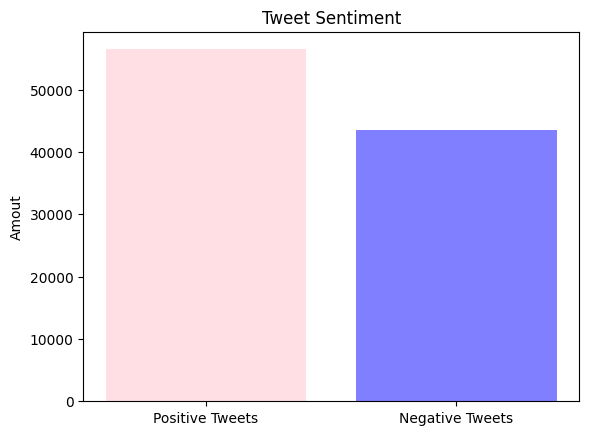
\includegraphics[scale=0.38]{output}
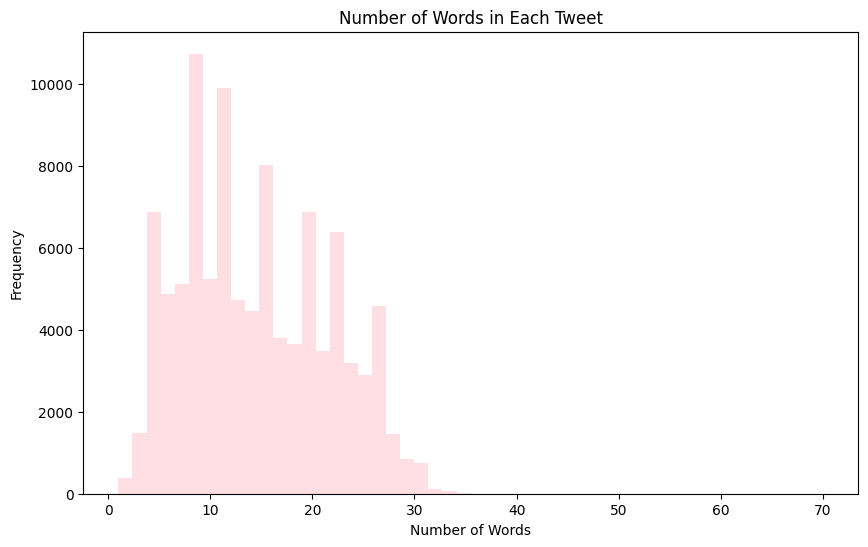
\includegraphics[scale=0.3]{numberofwords}
\centering
\end{figure}
\subsection{Preprocessing of the data}
The first step of our the pipeline is tokenization, which is the process of splitting the text into individual words or tokens. This is done using the "RegexTokenizer". The "inputCol" parameter is set to "SentimentText", which is the column in the DataFrame that contains the text to be tokenized.. The "pattern" parameter of the Tokenizer is set to "\\W", which means any non-word character is considered a delimiter. The second step in the pipeline is "stop words removal". Stop words are common words that do not carry much meaningful information and are often removed in text mining tasks. The "StopWordsRemover" class is used for this purpose. In order to eliminate all necessary stop words we imported the english stopwords corpus fromm nltk.corpus and added some custom stop words, like websites or hyperlinks. The third step in the pipeline is feature extraction. The "HashingTF" class converts all the words leftover after removing the stop words into numerical feature vectors.
To run these steps sequentially and have them contained in one object, we created a variable called pipeline. It includes all the steps mentioned above. This also makes it easier to rerun the pipeline if necessary. As mentioned in the introduction, our goal is to gain an overview of the extensive dataset provided.We want to create a Logistic Regression Model that can predict the sentiment of a tweet with at least 70\% accuracy. Additionally, we would like to understand the relationships between words used in tweets, such as identifying the words most likely used in the context of a tweet that also contains the word "happy."
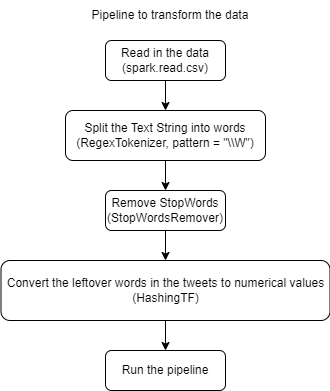
\includegraphics[scale = 0.5]{pipeline}
\subsection{Gensim, Word2Vec}
To find the word
\subsubsection{Dimensionreduction}
\subsection{A-priori to find words most often used together}
\subsection{Logistic Regression Model}
\subsubsection{Preparing the data for Logistic Regression}

\subsubsection{Training the model and applying it to the test-data}

\section{Results}
\section{Conclusion}
\section{References}







\end{document}
